\documentclass{article}

% packages
\usepackage{hyperref}
\usepackage{verbatim}
\usepackage{amsmath}
\usepackage{graphicx}
\usepackage{epstopdf}

% document style
\usepackage[margin = 20mm]{geometry}
\setlength\parindent{0pt}

\begin{document}

\section*{2HDM4TC Analysis Tutorial}

This tutorial guides the user through various stages of data simulation and analysis of the hypothetical process 
$p p \rightarrow{} A$, $A \rightarrow{} Z h$, $h \rightarrow{} b \bar{b}$, $Z \rightarrow{} l+ l-$ (henceforth, AZH).
In order to analyze aspects of this process such as its discovery potential for experiments such as ATLAS, we must also simulate and analyze the background process
$p p \rightarrow{} Z b \bar{b}$, $Z \rightarrow{} l+ l-$ (henceforth, PZB).
The prerequisites to this tutorial are a basic understanding of collider physics, Linux, C++, and ROOT. Refer to the following links for an overview of these topics.

\bigskip

collider physics:

Introduction to Collider Physics - \url{http://arxiv.org/abs/1002.0274}

...

\bigskip

This tutorial is broken up into 4 sections - Level 1, Level 2, Level 3, and Level 4.
In Level 1, you will install and configure the appropriate packages of ROOT, MadGraph,
Pythia, Delphes, and the 2HDM4TC Model in order to generate Montecarlo simulations of
our AZH process. You will also learn about each step in the Montecarlo simulation process,
that is, what exactly MadGraph, Pythia, and Delphes are doing, as well as how to edit
various configuration files to modify your simulation. Then, in Level 2, you will learn
how to analyze the truth particle data in the ROOT files generated by your simulation.
In Level 3, you will learn how to perform more extensive analysis on the detected particle
data in your ROOT files, both before and after various cuts. Finally, in Level 4, you will
learn how to manually analyze jets, with the motivation of creating a good jet reconstruction algorithm.

\bigskip

Before or concurrent to going through these Levels, you may want to look at slide presentations
of the Levels. They offer a broader and quicker overview of the Levels. They can be found in the
PhysAna-AtoZh git repository at the following url.

\bigskip

\url{https://github.com/schsu/PhysAna-AtoZh/tree/master/documentation/presentations}

\section{Level 1: Generating Simulated Events with MadGraph, Pythia, Delphes, and 2HDM4TC}

The 2HDM4TC model is a model for decays involving the heavy Higgs particle, referred to as A or h3.
This model currently does not work with the newest version of MadGraph, so there are some technical
complications in getting the model to work with MadGraph, Pythia, and Delphes. This section aims to
be a step-by-step manual for installing and configuring MadGraph, Pythia, Delphes, and the 2HDM4TC
model to create a working environment for heavy Higgs Montecarlo studies. The details of the Montecarlo
simulation are then discussed, and finally configuring the simulation is explained.

\subsection{Installing ROOT}

ROOT is a software package developed by CERN. It is used in most particle physics data analysis,
and is required here to both generate and analyze Events. To install it, first download it from
the following url using wget.

\begin{verbatim}
	wget ftp://root.cern.ch/root/root_v5.34.14.source.tar.gz
\end{verbatim}

Then untar it.

\begin{verbatim}
	tar -xzf root_v5.34.14.source.tar.gz
\end{verbatim}

Then cd to the untarred directory.

\begin{verbatim}
	cd root
\end{verbatim}

Then run ./configure.

\begin{verbatim}
	./configure
\end{verbatim}

And finally compile root with make.

\begin{verbatim}
	make
\end{verbatim}

Compiling root may take a very long time. After compiling root, you must run the
script thisroot.sh using the command source.

\begin{verbatim}
	source root/bin/thisroot.sh
\end{verbatim}

\subsection{Installing MadGraph}

MadGraph is the software package which does our Montecarlo simulation. It takes
process definitions and models as input, and outputs a process directory in which
you modify simulation settings and generate Events. We will go over using MadGraph
in detail later. For now, download it from the following url using wget.

\begin{verbatim}
	wget https://launchpad.net/mg5amcnlo/trunk/1.5.0/+download/MadGraph5_v1.5.14.tar.gz
\end{verbatim}

Then untar it.

\begin{verbatim}
	tar -xzf MadGraph5_v1.5.14.tar.gz
\end{verbatim}

\subsection{Installing Pythia}

Pythia generates particle showers from the partons generated by MadGraph.
This will be explained in more detail later. For now download Pythia to the
MadGraph directory from the following url using wget.

\begin{verbatim}
	wget http://madgraph.hep.uiuc.edu/Downloads/pythia-pgs_V2.2.0.tar.gz
\end{verbatim}

Then untar it.

\begin{verbatim}
	tar -xzf pythia-pgs_V2.2.0.tar.gz
\end{verbatim}

Then cd to the untarred directory.

\begin{verbatim}
	cd pythia-pgs
\end{verbatim}

Then cd to the src directory.

\begin{verbatim}
	cd src
\end{verbatim}

We need to edit the file "makefile" in this src directory. Find the following line in the makefile.

\begin{verbatim}
	Links = mass_width_2004.mc pgs clean_output PDFsets pydata.f
\end{verbatim}

And change it to the following.

\begin{verbatim}
	Links = mass_width_2004.mc PDFsets pydata.f
\end{verbatim}

Then cd back to pythia-pgs

\begin{verbatim}
	cd ..
\end{verbatim}

And finally compile pythia with make.

\begin{verbatim}
	make
\end{verbatim}

\subsection{Installing Delphes}

Delphes simulates the detector response to particle physics processes. It
is explained in more detail later. For now, download Delphes to the MadGraph
directory using the following url with wget.

\begin{verbatim}
	wget http://cp3.irmp.ucl.ac.be/downloads/Delphes-3.0.12.tar.gz
\end{verbatim}

Then untar it.

\begin{verbatim}
	tar -xzf Delphes-3.0.12.tar.gz
\end{verbatim}

Now change the untarred directory's name to "Delphes".

\begin{verbatim}
	mv Delphes-3.0.12 Delphes
\end{verbatim}

Finally, cd to Delphes and run "make".

\subsection{Installing 2HDM4TC Model}

The 2HDM4TC Model we use can be found in the git repository for this project.
To get it, first clone the repository:

\begin{verbatim}
	git clone https://github.com/schsu/PhysAna-AtoZh
\end{verbatim}

Then locate the model from the following directory in the repository:

\begin{verbatim}
	PhysAna-AtoZh/models/2HDM4TC.tar
\end{verbatim}

And copy it into your MadGraph directory. Finally, untar the model:

\begin{verbatim}
	tar -xzf 2HDM4TC.tar
\end{verbatim}

\subsection{MadGraph Explanation}

I ought to now explain the roles of these packages which you have installed. MadGraph is a Montecarlo Event simulator.
Given a series of files which define and configure a physical process, MadGraph will simulate the process and output
Events in an LHE file. MadGraph simulates physical processes at the parton (quarks and gluons) level. This means that quarks and gluons,
rather than QCD jets, show up in the output. Since we know that these particles do not exist in isolation in nature
(all nature particles are "colorless"), the simulation ought not end at this step.

\subsection{Pythia Explanation}

Pythia takes the LHE file generated by MadGraph and produces another LHE file and an HEP file as output.

\bigskip

Pythia performs the next step in our simulation - it simulates the parton showers that result from the accelerating
partons output from MadGraph. Partons carry color, so when they accelerate, they radiate gluons, which may decay
into other quarks, which may radiate more gluons, etc. Partons also can carry charge, and can thus radiate photons
which can decay into charged positive and negative leptons (pair production). The cascade of particles that
result from an accelerating parton is refered to as a parton shower. It is for this reason that Events which have
passed through Pythia's simulation contain many more particles than Events which have not.

\subsection{Delphes Explanation}

Delphes takes the HEP file generated by Pythia and produces a ROOT file as output. These ROOT files are the files
that we will use for our analysis.

\bigskip

Delphes simulates the detector response to the particles output from MadGraph and Pythia. One can imagine if a detector's 
geometry is that of a cylindrical shell (such as is the case with ATLAS), particles
with low PT and high Eta will not be detected. Also, when a particle is detected, the detector cannot exactly measure its
energy or momentum. In order to simulate these effects, Delphes will apply efficiencies to detecting particles as a function
of their PT and Eta, and apply energy and momentum smearing. Delphes also applies jet reconstruction algorithms and jet flavor
tagging (such as b-tagging, which we will be interested in).

\subsection{Modifying Configuration Files}

The configuration of our simulation is determined by a series of configuration
files, called "cards." MadGraph, Pythia, and Delphes all use several of these cards.
The most relevant cards for our simulations, and ones that you may have to edit frequently
in your analysis studies, are the process card, the parameter card, the run card, and the
Delphes card. I will go over their roles and how to edit them in the following sections.

\subsubsection{Process Card}

The first input for MadGraph to generate events is a process card. This card defines the
physical process simulated, such as our AZH process. When using a process which involves
Beyond Standard Model (BSM) particles and parameters, such as our A particle, the process
needs to reference a model. This is precisely why we need our 2HDM4TC model to simulate our AZH process.

\bigskip

For now, copy our AZH process card from the following url into your MadGraph directory.

\bigskip

\url{https://github.com/schsu/PhysAna-AtoZh/tree/master/Cards/proc-2HDM4TC-gg-h3-zh.dat}

\bigskip

You should open this process card to see what exactly is going on. In particlular, you will that it does use our 2HDM4TC model.

\begin{verbatim}
	import model_v4 2HDM4TC -modelname
\end{verbatim}

You will also see a series of definitions for particles such as the following.

\begin{verbatim}
	define lp e+ mu+
\end{verbatim}

MadGraph knows the definitions of e+ and mu+, but it does not define lp to mean either e+ or mu+.
That's what these define statements do. Finally, you'll see our process generated and output at
the end of the process card.

\begin{verbatim}
	generate g g > h3, (h3 > z h1, z > lp lm, h1 > b b~)
	output madevent proc-2HDM4TC-gg-h3-zh -f
\end{verbatim}

The output will all be in a folder called "proc-2HDM4TC-gg-h3-zh" - you may, of course, change this to whatever you like.

\bigskip

We will also need to produce Events of our background PZB process. Copy our PZB process card
from the following url into your MadGraph directory.

\bigskip

\url{https://github.com/schsu/PhysAna-AtoZh/tree/master/Cards/proc-std-pp-zbb.dat}

\bigskip

If you look in this process card, you will not see a reference to any model. This is because
our PZB process is a Standard Model process, and MadGraph already has cards defining all Standard Model parameters.

\subsubsection{Parameter Card}

The parameter card defines various physics parameters of a process. For example, it will contain the definition of coupling
constants and particle masses. Because our 2HDM4TC model is BSM, it contains its own parameter card, called "param\_card.dat" (located in your 2HDM4TC directory).
Because our AZH process card refers to our 2HDM4TC model, this parameter card will be copied into the process directory when
we use MadGraph to do our simulation.

\bigskip

You should look over this parameter card to understand what all is defined in it. In
particular, you should find where the mass of A is defined. Since A is a hypothetical partical, this mass is a free parameter
in our simulations, and we should study runs of Events for various masses of A, typically between 600 GeV and 3000 GeV.

\bigskip

Our background PZB process does not use the 2HDM4TC model, so it will not use this same parameter card. Instead, you will
find its parameter card in your MadGraph directory under Templates/Cards/param\_card.dat and Templates/Cards/param\_card\_default.dat.
These cards will be copied into your PZB process directory when we use MadGraph to simulate our PZB process. Take a look at this card
and make sure that the parameters shared between this card and the parameter card for our AZH process are the same. For example,
make sure that both cards are using 125 GeV for the mass of the SM Higgs.
Feel free to compare the parameter card for your background with the one I've been using for my simulations, located in the git repository at the following url.

\bigskip

\url{https://github.com/schsu/PhysAna-AtoZh/tree/master/Cards/pp-zbb/param_card.dat}

\bigskip

(Since the parameter card for your AZH process comes from the 2HDM4TC directory, it should already be identical to the one in the git repository.
It is located at the following url anywho.)

\bigskip

\url{https://github.com/schsu/PhysAna-AtoZh/tree/master/model/2HDM4TC/param_card.dat}

\subsubsection{Run Card}
\label{sec:runCard}

With the physical parameters of our process defined in the parameter card, and detector response parameters defined in the Delphes card (as you will see below),
parameters related to the data run we will be simulated are defined in the run card. While the term "run" when referring to data collection
is not consistently defined in physics, it typically refers to either a very short period of time in which data is continuosly collected (when bunches
of particles of particles enter a detector at an accelerator, for example) or the longer period of time in which a particular experiment collects data
(such as the LHC "Run 2").

\bigskip

Either way, during a run a certain number of "Events" are collected, and ideally the parameters of the data generating device (such as
an accelerator) are constant. As such, you will find that in a run card parameters such as the number of Events and beam energy are defined.
Look for these parameters in your run card (called run\_card.dat), located under Templates/Cards in your MadGraph directory.

\bigskip

You should change the number of Events to the largest number you can (for technical reasons, this happens to be 50000 if you intend to use Pythia).
The reason for generating so many Events is to have high statistics. When counting Events which pass certain cuts, for example, the uncertainty of
the resulting number is the square root of the number of counted Events (we say our data is "Poisson distributed"). Thus, the more Events we have
in general, the lower our uncertainties will be (if we count 100 Events, for example, our uncertainty would be 10 percent, if we count 10000 Events,
on the other hard, our uncertainty would be only 1 percent).

\bigskip

You may also want to change your beam energy to reflect either past runs at the LHC (4000 GeV per beam), or future runs at the LHC (7000 GeV per beam), for example.
Feel free to compare your run card with the one I've been using for my simulations, located in the git repository at the following url.

\bigskip

\url{https://github.com/schsu/PhysAna-AtoZh/tree/master/Cards/run_card.dat}

\bigskip

Now, there is one more set of parameters we will need to edit at some point in our simulations - the parameters "ihtmin" and "ihtmax".
ihtmin and ihtmax refer to the minimum and maximum PT for partons generated by MadGraph. In our AZH process, we should not have bounds
on our partons' PT, but for our PZB process we will need generate data runs for several ranges of parton PT. The reason for this is
that in our PZB process, we expect most Events to produce partons with very low PT (you can always generate PZB Events without bounding
your parton PT to see this for yourself), whereas in our AZH process, the partons generated (our b quarks) come from the 125 GeV Higgs decaying,
so we would expect our Events to contain partons with very high PT.

\bigskip

This distinction is good in a sense - it allows us to differentiate between
our processes, allowing us to calculate signal vs background efficiencies - but it is bad in another sense - having very few background Events
with high parton PT will result in large error bars and low statistics. In order to get around this, we can force our simulation to generate
many Events for various ranges of parton PT, using the ihtmin and ihtmax variables.

\bigskip

For example, for our background PZB process, let's generate
50000 Events for each 100 GeV range of parton PT - that is, 50000 Events with parton PT in the range 0 GeV to 100 Gev, 50000 Events with parton
PT in the range 100 GeV to 200 GeV, etc, all the way up to the mass of A used in the AZH process. We can later normalize our distribution without
sacrificing the good statistics gained by generating so many Events.

\subsubsection{Delphes Card}

The version of MadGraph you have installed is an older version because the 2HDM4TC model does
not work with the newer version of MadGraph. As a result, the Delphes card which comes in your

\begin{verbatim}
	MadGraph5_v1_5_14/Template/Cards
\end{verbatim}

directory will not produce the correct output for our study. When preparing a process for
simulation, MadGraph creates a process directory and copies the cards from this Template/Cards
directory into the Cards directory for your process. Thus, all processes you generate will by
default use the Delphes card in the Template/Cards directory.

\bigskip

For now, replace delphes\_card\_default.dat in MadGraph5\_v1\_5\_14/Template/Cards with the Delphes card from the following url

\bigskip

\url{https://github.com/schsu/PhysAna-AtoZh/tree/master/Cards/delphes_card_default.dat}

\bigskip

You should read through this Delphes card to become familiar with some of the modules it uses. A "module" is a like a function which Delphes executes
when applying the detector response and jet reconstruction. At the beginning of our Delphes card is a section called ExecutionPath which defines
the order in which modules will be executed. You can see that Delphes will call efficiency, energy smearing, momentum smearing, and jet finding modules,
among others. You should take a look at the definitions of these modules, as they define important detector response parameters such as the efficiency
of detecting particular particles. When analyzing the output of Delphes, it is important to verify that your simulation behaved as expected, so you may
want to cross check the efficiency of detecting particles in your output vs what is defined in your Delphes card. Some of these verifications are discussed
farther in the tutorial.

\subsection{Generating Your Simulation}

Now you should be ready to generate your simulation! With all the cards in the right places, cd to your MadGraph directory and run the following command.

\begin{verbatim}
	./bin/mg5 proc-2HDM4TC-gg-h3-zh.dat
\end{verbatim}

This should create a process directory called proc-2HDM4TC-gg-h3-zh - cd to this directory and run the following command.

\begin{verbatim}
	./bin/generate_events
\end{verbatim}

This should bring up a prompt asking you exactly which steps you would like to carry out in
your simulation. There should be an option to use Delphes - the last step in our simulation.
Pick this option, and your simulation should be underway!

\bigskip

The Events generated should be output into a ROOT file under "Events/run\_01" in your
process directory. If you run the simulation again, the resulting output will be in a
ROOT file under "Events/run\_02" - so you can run the simulation as many times as you
want, possibly changing the parameter and run cards inbetween simulations to study different simulations.

\bigskip

You should, of course, repeat these steps to generate ROOT files for your PZB background Events. Remember
to edit the ihtmin and ihtmax variables in your run card, as discussed in Section \ref{sec:runCard}, in order to create the desired
amount of background Events for good statistics later on.

\subsubsection*{Exercises}

You will need to simulate Events for various ranges of parton PT for the PZB process and various ranges of the mass of A for the AZH process.
It would be worth writing a bash script to accomplish this in an automated fashion, as the simulations may take some time.
You could run all the simulations overnight on your computer, or take advantage of the parallel computing offered by UW's TeV Cluster
and perform all simulations in roughly 10 minutes.

\section{Level 2: Truth Particle Study}

Before diving into analysis code, you will need to set up some shell environment variables in order to link to
Delphes and ROOT libraries. On my system, I have exported the following paths.

\begin{verbatim}
	export ROOTSYS=$HOME/Research/ATLAS/Analysis/root
	export PATH=$PATH:$ROOTSYS/bin
	export LD_LIBRARY_PATH=$LD_LIBRARY_PATH:$ROOTSYS/lib
	export DELPHESPATH=$HOME/Research/ATLAS/Analysis/MadGraph5_v1_5_14/Delphes
	export LD_LIBRARY_PATH=$LD_LIBRARY_PATH:$DELPHESPATH
\end{verbatim}

I suggest you do the same. You can edit your bashrc or bash\_profile file with these exports in order to have your
shell execute them on every start up.

\bigskip

Now, after generating Events following the procedure of Level 1, you should be ready to use
ROOT to analyze your output data. The first analysis we will do on the output ROOT files
is that of our truth particles. Studying the truth particles in our data will reveal the
structure of our Events, and understanding the kinematics of our truth particles is critical
in understanding the physical properties of our process, before the simulation of the detector
response performed by Delphes.

\bigskip

The goal, then, of Level 2 is to learn how to use ROOT to analyze the truth particles in our
data. This is accomplished via 2 programs, truth\_table and truth\_histogram.

\subsection{truth\_table}

truth\_table is a program which takes a ROOT file containing a Particle branch
as input, and outputs a table of information about the particles in the Particle
branch. Our simulation from Level 1 was configured to output all truth particles
from each step of the simulation to the Particle branch in our final ROOT files.

\bigskip

The code for truth\_table is located at the following url in the PhysAna-AtoZh git repository.

\bigskip

\url{https://github.com/schsu/PhysAna-AtoZh/tree/master/level2/truth_table}

\bigskip

To compile and run it, run

\begin{verbatim}
	make
\end{verbatim} 

in the truth\_table directory and then run

\begin{verbatim}
	./truth_table
\end{verbatim}

The program should output the following usage statement.

\begin{verbatim}
	usage: ./truth_table inputFile [event] [numberofParticles]
\end{verbatim}

The program requires the user to provide the path to a ROOT file as commandline input.
When running the program with such a ROOT file, the program will display the number of
Events in the ROOT file and prompt the user for an Event to analyze. After providing an
Event to analyze, the program will display the number of truth particles in the Particle
branch of that Event, and prompt the user for a number of particles to analyze. After
providing the program with the number of particles to analyze, the program will output
a table of information for that number of particles.

\bigskip

To skip these interactive steps, you can supply the Event number and the number of
particles to analyze with the optional commandline arguments [event] and [numberofParticles].
An example output of truth\_table is displayed in Figure \ref{fig:truthTableOutput}.

\begin{figure}[h]
	\centering
	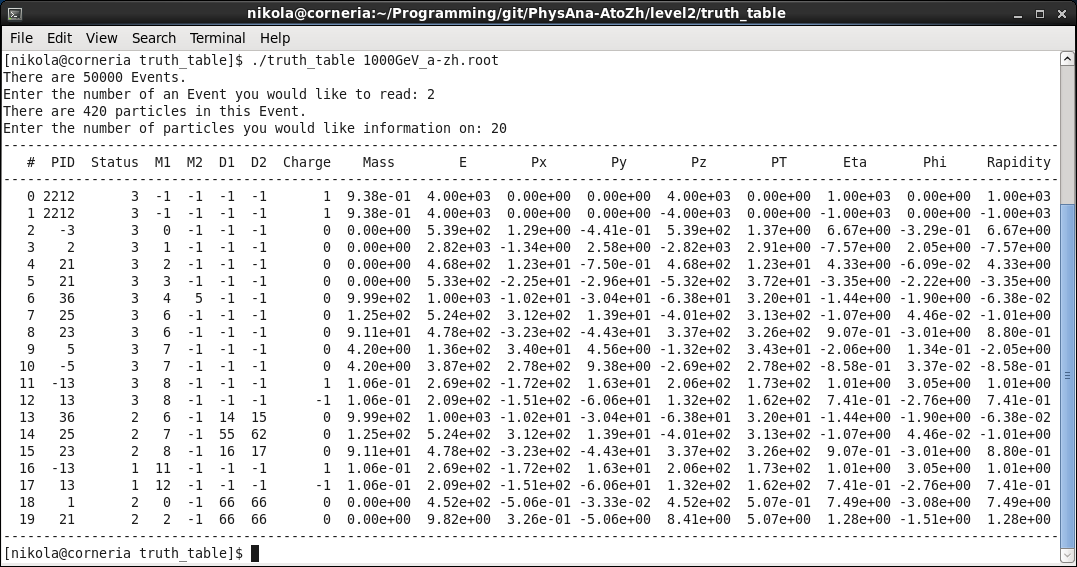
\includegraphics[width = \linewidth]{truth_table_screenshot.png}
	\caption{truth\_table Output}
	\label{fig:truthTableOutput}
\end{figure}

\bigskip

Before analyzing Figure \ref{fig:truthTableOutput}, it is worth taking a look at the code for
truth\_table in the main.cpp file in the truth\_table directory. With a basic understanding of
ROOT and C++, this code should be straight forward. However, you may want to play around with
which branches to read data from. For example, the code can be easily modified to read the
Electron branch of our ROOT files instead of the Particle branch, and to output a table of
information about the Electron objects in the Electron branch. To do this, for example, you
could simply change the line

\begin{verbatim}
	TClonesArray * branchParticle = tr->UseBranch("Particle");
\end{verbatim}

to something like

\begin{verbatim}
	TClonesArray * branchElectron = tr->UseBranch("Electron");
\end{verbatim}

Then you could loop through the Electron objects in this branch and output their information
using something like the following.

\begin{verbatim}
	for (int64_t i = 0; i < branchElectron->GetEntries(); i++)
	{
	        Electron * electron = (Electron*) branchElectron->At(i);

	        cout << electron->PT;

	        ...
	}
\end{verbatim}

Doing these small programming exercises will help to familiarize yourself with this type of
analysis programming, and make reading and modifying future larger analysis programs easier.
You are encouraged at any point throughout this tutorial to experiment with modifying the source
code of the tutorial programs, and will indeed have to to carry out some of the analysis exercises
presented here, or your own analysis.

\bigskip

Now, let's return to Figure \ref{fig:truthTableOutput}, and analyze each piece of the output truth
particle information to understand the structure of a truth particle and of our Event.

\bigskip

The physical variables, such as Mass and E, should be evident. However, I should clarify the
meaning of \#, PID, Status, M1, M2, D1, and D2.

\subsubsection{\#}

\# simply refers to the index of a particle. The Particle branch in our ROOT files contain an
array of GenParticle objects, each object corresponding to a truth particle. \# here refers to
the index of a truth particle in that array. You can see in the code for truth\_table that we
are outputting our truth particle information starting from the first index in the GenParticle array.

\subsubsection{PID}

PID stands for "Particle ID." Each particle, such as electrons, anti muons, protons, etc, is
identified here by an integer. For example, 13 refers to muons and 23 refers to Z bosons. A
complete list of the PIDs for various particles is available at the following url.

\bigskip

\url{http://www.physics.ox.ac.uk/CDF/Mphys/old/notes/pythia_codeListing.html}

\subsubsection{Status}

The Status of a particle can be either 3, 2, or 1. Status 3 refers to truth particles output
from MadGraph, before parton showers are simulated by Pythia. Thus, for our AZH process, we
would expect there to be exactly 2 Status 3 electrons or exactly 2 Status 3 muons. In the table
output above, we can see that there are indeed exactly 2 Status 3 muons (2 Status 3 particles
with PID 13). (You may be wondering if there are more Status 3 particles listed later in the
table, as the table only lists the first 20 truth particles. You can verify for yourself with
the program that all Status 3 particles occur at the beginning of the GenParticle array.) Status
2 particles are intermediate between Status 3 and Status 1 particles. Status 1 particles are final
state particles - these are the truth particles left over at the end of the MadGraph and Pythia
simulation processes (but before the Delphes detector response simulation, of course).

\subsubsection{M1, M2, D1, and D2}

M1, M2, D1, and D2 refer to the indices of the mother and daughter particles of a particle.
For example, we can see in Figure \ref{fig:truthTableOutput} that the index of the mother particle
of particle \#12 (a muon) is particle \#8 (a Z boson). Using these variables, you can scan through
a table to see the decay chains of all truth particles. You can do this either by eye, or by writing a program.

\subsubsection*{Exercises}

As an exercise at this point, you could write a program to count up all truth electrons in an Event,
and use the M1 and M2 member variables to find the ultimate mother particle of these electrons. You can
verify that the ultimate mother of all electrons is one of the Status 3 particles from the original MadGraph process.

\subsection{truth\_histogram}

The program truth\_histogram takes a ROOT file with a Particle branch as input, and outputs a histogram
of the PT distribution of all Status 1 electrons (PID 11) and positrons (PID -11) in the Particle branch.

\bigskip

The code for truth\_histogram is located at the following url in the PhysAna-AtoZh git repository.

\bigskip

\url{https://github.com/schsu/PhysAna-AtoZh/tree/master/level2/truth_table}

\bigskip

To compile and run it, run

\begin{verbatim}
	make
\end{verbatim} 

in the truth\_histogram directory and then run

\begin{verbatim}
	./truth_histogram
\end{verbatim}

The program should output the following usage statement.

\begin{verbatim}
	usage: ./truth_histogram inputFile
\end{verbatim}

The program requires the user to provide the path to a ROOT file as commandline input.
The program is not interactive - it just outputs the file "truth\_electron\_pt.eps" in
present working directory. The output EPS file should look something like Figure \ref{fig:truthElectron1PT}.

\begin{figure}[h]
\begin{minipage}{0.45\textwidth}
	\centering
	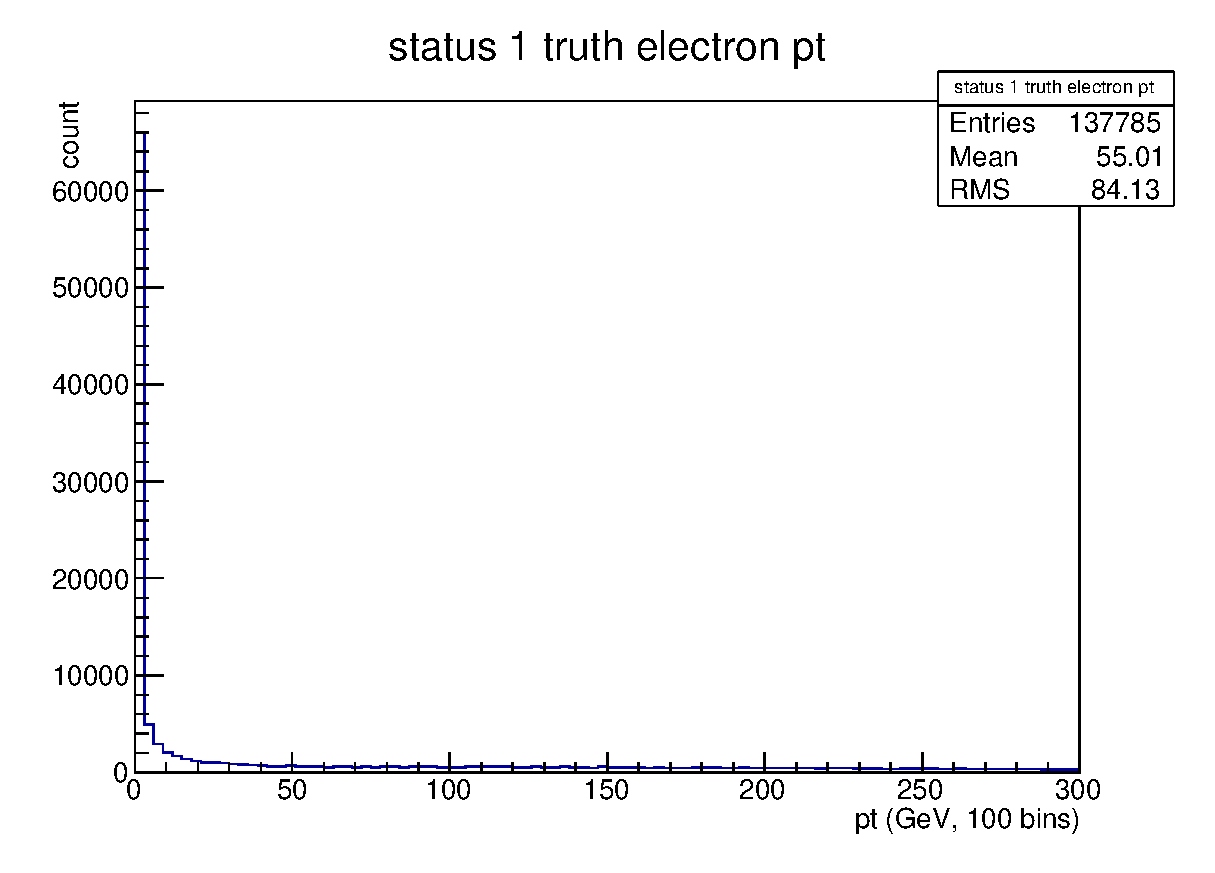
\includegraphics[width = \linewidth]{truth_electron_1_pt.eps}
	\caption{Here we see the PT distribution for Status 1 electrons. Notice how there are many electrons with low PT. This is because most final state electrons are actually produced in our parton shower simulation.}
	\label{fig:truthElectron1PT}
\end{minipage}
\hspace{0.1\textwidth}
\begin{minipage}{0.45\textwidth}
	\centering
	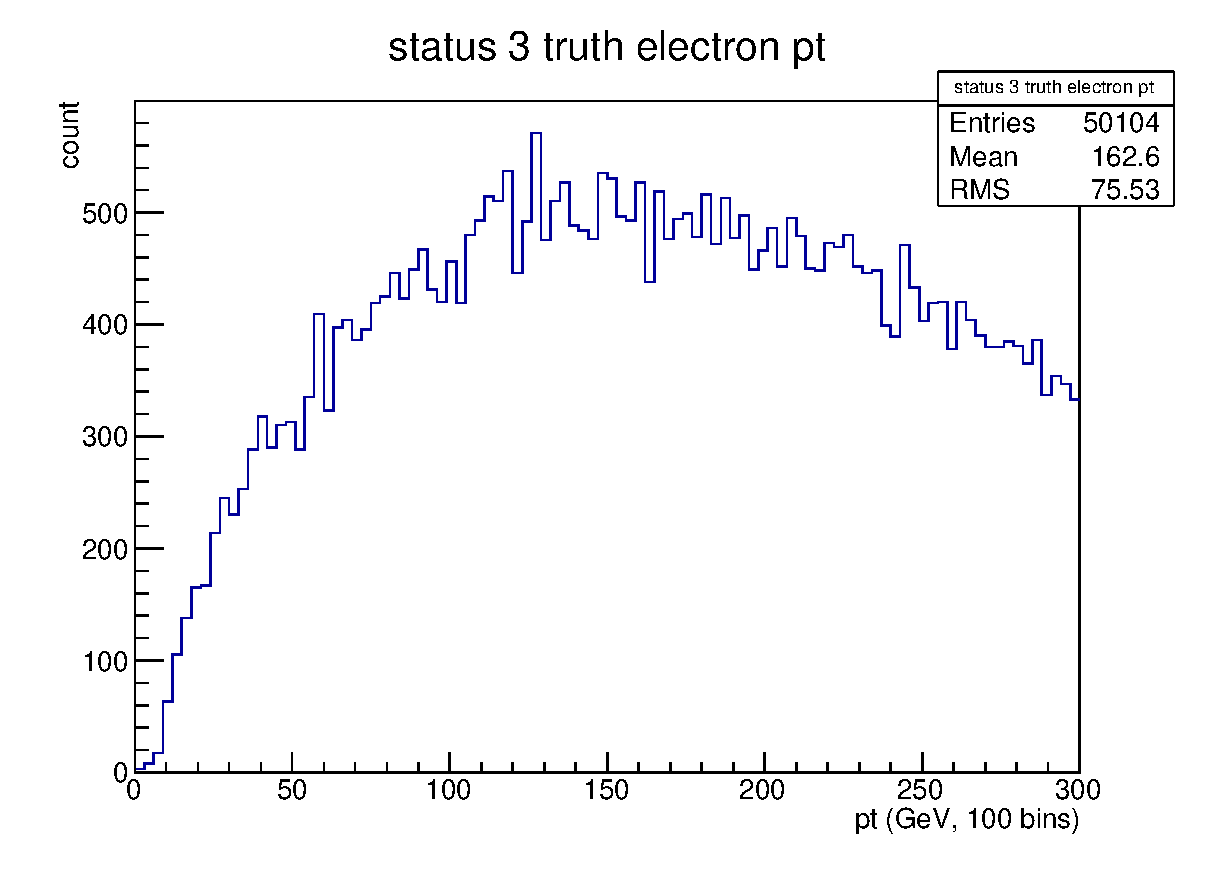
\includegraphics[width = \linewidth]{truth_electron_3_pt.eps}
	\caption{Here we see the PT distribution for Status 3 electrons. Notice how there are many electrons with high PT. This is because Status 3 electrons in our simulation are decay products of our Z boson.}
	\label{fig:truthElectron3PT}
\end{minipage}
\end{figure}

\bigskip

Now we are ready to make some real physics analysis plots! The source code for truth\_histogram
is very short, so it should be very easy to modify to output truth particle histograms of whatever
you may be interested in - Status 1 electron PT, Status 3 muon energy, Status 3 Z boson Eta, you
name it. For now, let's discuss the plot in Figure \ref{fig:truthElectron1PT}, and some real physics for a moment.

\bigskip

We see in Figure \ref{fig:truthElectron1PT} that the vast majority of Status 1 electrons have
very low PT. However, the AZH process we are trying to analyze should produce 2 electrons (or muons)
which decay from a Z boson. The Z boson has a mass of around 90 GeV, while an electrons only has a
mass of 0.05 GeV, so the vast majority of the Z boson's mass should go into the electrons momentum.
Thus, we should expect our electrons to have high PT. Why, then, do most of our Status 1 electrons
have low PT? To answer that, let's first plot the PT distribution of Status 3 electrons. We know
that Status 3 electrons are the electrons which decayed from our Z boson, whereas Status 1 electrons
may have been produced by our parton shower. This plot is displayed in Figure \ref{fig:truthElectron3PT}.

\bigskip

Indeed, we see that Status 3 electrons have a high PT distribution! In fact, we see that there are
much less Status 3 electrons in our Particle branch than Status 1 electrons. This should make sense
after studying the truth\_table program and its output. Now we can ask ourselves, does it make sense
that electrons produced by our parton showers have low PT? ...

\bigskip

Understanding these plots is at the heart of physics analysis. These PT distributions offer early
motivation for a low PT cut, however, since we are studying truth particle information, and not
detected particles (the step performed by Delphes), it is a bit too early to discuss cuts. This
is left for Level 3 of this tutorial.

\subsubsection*{Exercises}

An example of real physics analysis was presented with comparing the PT distribution of Status
3 and Status 1 electrons. With very slight modifications to the truth\_histogram code, you could
at this point study many kinematic aspects of our truth particles. For example, you could study
the opening angle distribution of the 2 electrons (or muons) which decay from our Z boson, or
maybe make a 2D histogram of this opening angle distribution vs combined PT of the 2 electrons
(or muons). You could also verify that the mass of the combined electrons' 4vector is indeed
the mass of our Z boson. You could similarly verify that the combined 4vector mass of the 2
bottom quarks which decayed from our Higgs is indeed the mass of our Higgs. You could study
the opening angle distribution of our Higgs and our Z boson which decayed from A. Being able
to produce these plots is critical in all following analysis, and you should feel free to both
practice producing these plots, and thinking up good questions which could be answered by viewing these plots.

\section{Level 3: Detected Particle Study}

\end{document}
